\begin{figure}[t]
  \centering
  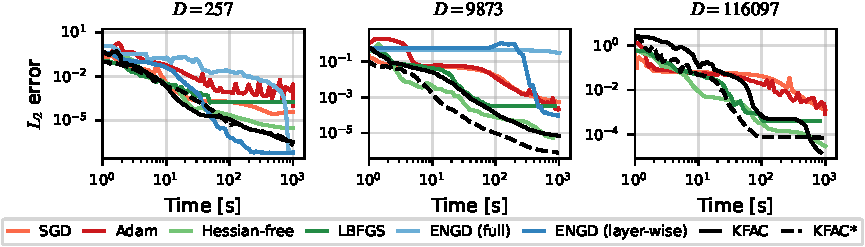
\includegraphics{../kfac_pinns_exp/exp17_groupplot_poisson2d/l2_error_over_time.pdf}
  \caption{Performance of different optimizers on the 2d Poisson equation~\eqref{eq:2D-Poisson} measured in relative $L_2$ error against wall clock time for architectures with different parameter dimensions $D$.}
  \label{fig:2D-Poisson}
\end{figure}

We implement KFAC, KFAC*, and ENGD with either the per-layer or full Gramian in PyTorch~\citep{paszke2019pytorch}.
As a matrix-free version of ENGD, we use the Hessian-free optimizer~\citep{martens2010deep} which uses truncated conjugate gradients (CG) with exact Gramian-vector products to pre-condition the gradient.
We chose this because there is a fully-featured implementation from~\citet{tatzel2022late} which offers many additional heuristics like adaptive damping, CG backtracking, and backtracking line search, allowing this algorithm work well with little hyper-parameter tuning.
As baselines, we use SGD with tuned learning rate and momentum, Adam with tuned learning rate, and L-BFGS with tuned learning rate and history size.
We tune hyper-parameters using Weights \& Biases~\citep{wandb} (see \Cref{sec:tuning-protocol} for the exact protocol).
For random/grid search, we run an initial round of 50 runs with generous search spaces, then narrow them down and re-run for another 50 runs; for Bayesian search, we assign the same total compute to each optimizer.
We report the runs with lowest $L_2$ error approximated on a held-out data set and using the known solution to the studied PDEs.
To be comparable, all runs are executed on a compute cluster with RTX 6000 GPUs (24\,GiB RAM) and in double precision, and we use the same computation time budget for all optimizers on a fixed PINN problem.
All search spaces and best run hyper-parameters, as well as training curves over iteration count rather than time, are in \Cref{sec:experimental_details}.

\textbf{Pedagogical example: 2d Poisson equation}
We start with a low-dimensional Poisson equation from~\citet{muller2023achieving} to reproduce ENGD's performance (\Cref{fig:2D-Poisson}).
It is given by
\begin{align}\label{eq:2D-Poisson}
  \begin{split}
    -\Delta u(x,y) & = 2\pi^2 \sin(\pi x) \sin(\pi y) \quad \text{for } (x,y)\in[0,1]^2 \\
    u(x,y) & = 0 \quad \text{for } (x,y) \in\partial[0,1]^2.
  \end{split}
\end{align}
Like the original paper, we choose a fixed data set of identical batch size for training, then use random/grid search to evaluate the performance of all optimizers for different $\tanh$-activated MLPs, one shallow and two with five fully-connected layers of different width (all details in \Cref{sec:2d-poisson-appendix}).
We include ENGD whenever the network's parameter space is small enough to build up the Gramian.

For the shallow net (\Cref{fig:2D-Poisson}, left), we can reproduce the results of~\cite{muller2023achieving}, where exact ENGD achieves high accuracy.
In terms of computation time, our KFACs are competitive with full-ENGD for a long phase, outperforming the first-order and quasi-Newton baselines.
In contrast to ENGD which runs out of memory for networks with more than $\num{10000}$ parameters, KFAC scales to larger networks (\Cref{fig:2D-Poisson}, middle/center) and is competitive to other second-order optimizers like Hessian-free, which uses more sophisticated heuristics.
We make similar observations on a (1+1)d heat equation with the same models, see \Cref{sec:1d-heat-equation,fig:heat1d-appendix}.

\begin{figure}
  \centering
  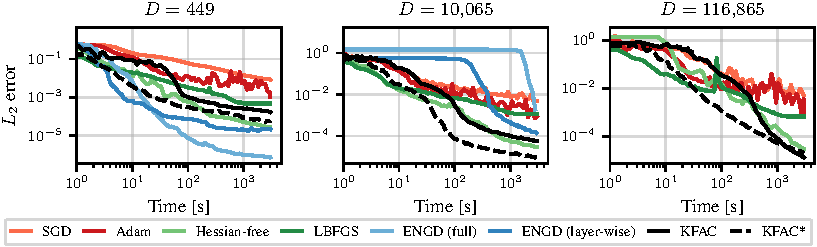
\includegraphics{../kfac_pinns_exp/exp30_heat4d_groupplot/l2_error_over_time.pdf}
  \caption{Performance of different optimizers on the (4+1)d heat equation~\eqref{eq:4D-heat} measured in relative $L^2$ error against wall clock time for architectures with different parameter dimensions $D$.}
  \label{fig:4D-heat}
\end{figure}

\textbf{An evolutionary problem: (4+1)d heat equation}
To demonstrate that our methods can also be applied to other problems than the Poisson equation, we consider a four-dimensional heat equation
\begin{align}\label{eq:4D-heat}
  \begin{split}
    \partial_t u(t,\vx)-\kappa\Delta_\vx u(t,\vx)
    &=
      0 \quad \text{for } t\in[0,1], \vx\in [0,1]^{4}\,,
    \\
    u(0,\vx)
    &=
      \textstyle
      \sum_{i=1}^{4} \sin(2 x_i) \quad \text{for }
      \vx\in [0,1]^{4}\,,
    \\
    u(t,\vx)
    &=
      \textstyle
      \exp(-t) \sum_{i=1}^{4} \sin(2 x_i) \quad \text{for } t\in[0,1], \vx\in\partial[0,1]^{4}\,,
  \end{split}
\end{align}
with diffusivity constant $\kappa = 1/4$, similar to that studied in \cite{muller2023achieving} (see \Cref{sec:pinn-loss-heat-equation} for the heat equation's PINN loss).
We use previous architectures with same hidden widths and evaluate optimizer performance with random/grid search(all details in \Cref{sec:4d-heat-app}), see \Cref{fig:4D-heat}.
To prevent over-fitting, we use mini-batches and sample a new batch each iteration.
We noticed that KFAC improves significantly when batches are sampled less frequently and hypothesize that it might need more iterations to make similar progress than one iteration of Hessian-free or ENGD; consequently we sample a new batch only every 100 iterations for KFAC.
To ensure that this does not lead to an unfair advantage for KFAC, we conduct an additional experiment for the MLP with $D=\num{116864}$ where we tune batch sizes, batch sampling frequencies, and all hyper-parameters with generous search spaces using Bayesian search (\Cref{sec:4d-heat-bayes-app}).
We find that this does not significantly boost performance of the other methods (compare \Cref{fig:4D-heat,fig:heat4d-bayes-appendix}).
Again, we observe that KFAC offers competitive performance compared to other second-order methods for networks with prohibitive size for ENGD and consistently outperforms SGD, Adam, and L-BFGS. We confirmed these observations with another 5d Poisson equation on the same architectures, see~\Cref{sec:poisson5d-appendix,fig:poisson5d-appendix}.

\begin{figure}
  \centering
  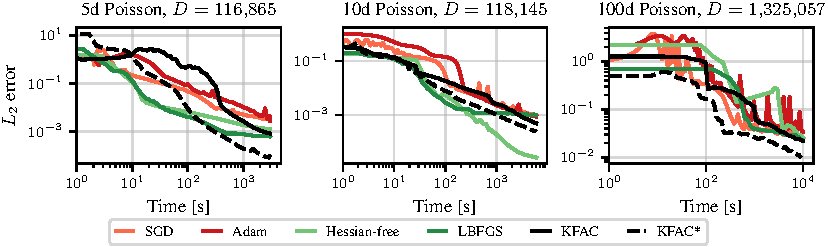
\includegraphics{../kfac_pinns_exp/exp33_poisson_bayes_groupplot/l2_error_over_time.pdf}
  \caption{
    Optimizer performance on Poisson equations in high dimensions and different boundary conditions measured in relative $L_2$ error against wall clock time for networks with $D$ parameters.
  }
  \label{fig:10D-Poisson}
\end{figure}

\textbf{High-dimensional Poisson equations}
To demonstrate scaling to high-dimensional PDEs and even larger neural networks, we consider three Poisson equations ($d=5,10,100$) with different boundary conditions used in~\cite{yu2018deep, muller2023achieving}, which admit the solutions
\begin{align}\label{eq:solutions_poisson}
  \begin{split}
    u_\star(\vx)
    &=
      \textstyle
      \sum_{i=1}^5 \cos(\pi x_i) \quad \text{for } \vx\in [0,1]^{5}\,,
    \\
    u_\star(\vx)
    &=
      \textstyle
      \sum_{k=1}^5 x_{2k-1}x_{2k},  \quad \text{for } \vx\in [0,1]^{10}\,,
    \\
    u_\star(\vx)
    &=
     \lVert \vx \rVert_2^2 \quad \text{for } \vx\in [0,1]^{100}\,,
  \end{split}
\end{align}
using the same architectures as before, but with larger intermediate widths and parameters up to a million (\Cref{fig:10D-Poisson}).
Due to lacking references for training such high-dimensional problems, we select all hyper-parameters via Bayesian search, including batch sizes and batch sampling frequencies (all details in \Cref{sec:high-dimensional-poissons-app}).
We see a similar picture as before with KFAC consistently outperforming first-order methods and offering competitive performance among second-order methods.
To account for the possibility that the Bayesian search did not converge properly to the best hyper-parameters, we conduct a random/grid search experiment for the 10d Poisson equation (\Cref{fig:10D-Poisson}, middle) in \Cref{sec:poisson10d-appendix}, using the same batch sizes and batch sampling frequencies as for the $(4+1)$d heat equation. In this experiment, KFAC further improved and achieved the same final performance as Hessian-free, see
\Cref{TODO}.

%%% Local Variables:
%%% mode: latex
%%% TeX-master: "../main"
%%% End:
